% --------------------------------------------------------------
% This is all preamble stuff that you don't have to worry about.
% Head down to where it says "Start here"
% --------------------------------------------------------------

\documentclass[12pt]{article}

\usepackage[nouppercase,headsepline,footsepline,plainfootsepline]{scrpage2}
\automark{section}
\pagestyle{scrheadings}
%\clearscrheadfoot
\ihead{{\bf Math 632}: Poisson Process\;\;Nov 06}
%\ofoot[\pagemark]{\pagemark}% Optional argument controls chapter-starting pages
\ifoot[(Author)]{{\sl \hfill Meenmo K.}}

\usepackage[margin=1in]{geometry}
\usepackage{amsmath,amsthm,amssymb,scrextend}
\usepackage{fancyhdr}
\usepackage{enumitem}
\usepackage{amsmath}
\usepackage{amssymb}
\usepackage{textcomp}
\usepackage{fancybox}
\usepackage{tikz}
\usepackage{cancel}
\usepackage{tasks}


\newcommand{\N}{\mathbb{N}}
\newcommand{\Z}{\mathbb{Z}}
\newcommand{\I}{\mathbb{I}}
\newcommand{\R}{\mathbb{R}}
\newcommand{\Q}{\mathbb{Q}}
\renewcommand{\qed}{\hfill$\blacksquare$}
\let\newproof\proof
\renewenvironment{proof}{\begin{addmargin}[1em]{0em}\begin{newproof}}{\end{newproof}\end{addmargin}\qed}
% \newcommand{\expl}[1]{\text{\hfill[#1]}$}
\setlength{\parindent}{0pt}
\newenvironment{theorem}[2][Theorem]{\begin{trivlist}
\item[\hskip \labelsep {\bfseries #1}\hskip \labelsep {\bfseries #2.}]}{\end{trivlist}}
\newenvironment{lemma}[2][Lemma]{\begin{trivlist}
\item[\hskip \labelsep {\bfseries #1}\hskip \labelsep {\bfseries #2.}]}{\end{trivlist}}
\newenvironment{problem}[2][Problem]{\begin{trivlist}
\item[\hskip \labelsep {\bfseries #1}\hskip \labelsep {\bfseries #2.}]}{\end{trivlist}}
\newenvironment{exercise}[2][Exercise]{\begin{trivlist}
\item[\hskip \labelsep {\bfseries #1}\hskip \labelsep {\bfseries #2.}]}{\end{trivlist}}
\newenvironment{reflection}[2][Reflection]{\begin{trivlist}
\item[\hskip \labelsep {\bfseries #1}\hskip \labelsep {\bfseries #2.}]}{\end{trivlist}}
\newenvironment{proposition}[2][Proposition]{\begin{trivlist}
\item[\hskip \labelsep {\bfseries #1}\hskip \labelsep {\bfseries #2.}]}{\end{trivlist}}
\newenvironment{corollary}[2][Corollary]{\begin{trivlist}
\item[\hskip \labelsep {\bfseries #1}\hskip \labelsep {\bfseries #2.}]}{\end{trivlist}}


\begin{document}
\begin{section}{\bf Poisson Process}
$$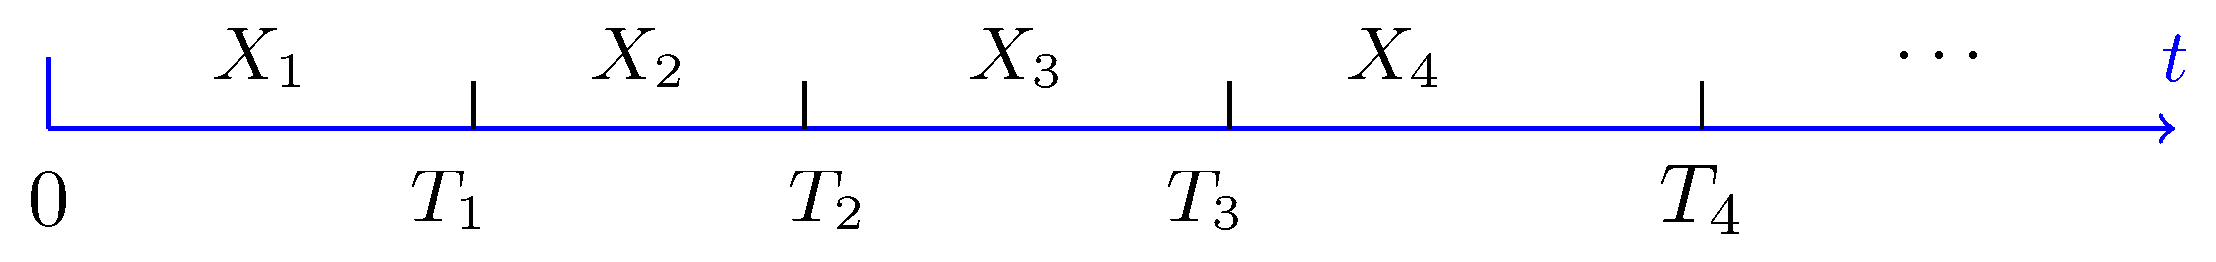
\includegraphics[height=1.5cm, width=13cm]{Poisson.png}$$

\begin{itemize}
    \item $N(t)$: The number of arrivals in $[0,t]$.
    \item $N(I)$: The number of arrivals in $I\subset [0,\infty)$.
\end{itemize}

Characterization
\begin{itemize}
    \item iid
    \item $N(b)-N(a)\sim $Poisson($\lmabda(b-a))$\\
    $N(s_1),\;N(s_2)-N(s_1),\ldots, N(s_n)-N(s_{n-1})$ are independent
\end{itemize}

\subsection{Thinking Property}
$N(t)$ is a Poisson process with rate $\lmabda$. We assign a type $Y_j \in \{1,2,,\ldots,l\}$ for the $j^{th}$ arrival. We assume that $Y_1,Y_2,\ldots,$ are $iid.$\\

Let $N_j(t)$ be the number of arrivals with type $J$ in $[0,t]$. Then $N_j$ is a Poisson process of rate $P_j\cdot d$. $N_1,N_2,\ldotsN_j$ are independent.

\subsubsection{Example}
Vehicles arrive at a roll both with a rate of $2/min$. The probability that a given vehicles is a truck is 2/3.
\begin{enumerate}[label=(\alph*)]
    \item P(exactly 2 cars and 3 trucks arriving in the next 5 minutes)
    \begin{itemize}
        \item Arriving vehicles form a Poisson process with rate $\lambda=2$.
        \item Let $N_1$ be the number of arrivals of trucks and $N_2$ be that of arrivals of cars.
        \item Then, for trucks, the rate of Poisson process is $\frac{2}{3}\lambda$ and the rate of Poisson process for cars is $\frac{1}{3}\lambda$.
        \item So $P(N_1(5)=3,\;N_2(5)=2)=P(N_1(5)=3)P(N_2(5)=2) = \frac{(\frac{20}{3})^3}{3!}e^{-\frac{20}{3}}\cdot \frac{(\frac{10}{3})^2}{2!}e^{-\frac{10}{3}}$

    \end{itemize}

    \item P(First arrival is a truck and the second one is a car) = $\frac{2}{3}\cdot \frac{1}{3}$
    \item Given that 20 trucks arrived in an hour what is expected the number of cars within the same hour? $\frac{1}{3}\cdot 60 = 20$\\
    
    The given 20 trucks actually does not affect the expected number of cars within the same time period.
\end{enumerate}

\subsection{Superposition Property}

Suppose that $N_1,\;N_2,\ldots,N_j$ are independent Poisson processes with the rate of $N_j$ is $\lambda_j$. We look at the union of all arrivals. This process is also a Poisson process, the rate $\lambda_1+\lambda_2+\ldots+\lambda_j$. The types of the arrivals will form an iid sequence where the probability of type $j = \frac{\lambda_j}{\lambda_1+\ldots+\lambda_j}$.

\vspace{1\baselineskip}
{\sl Proof.} Let $N_j$ be a counting functino of the $j^{th}$ Poisson process. Denote by $N$ the counting function of arrivals $N(t)=N_1(t)+N_2(t)+\ldots+N_j(t)$

$$N(b)-N(a)=\sum\limits_{j=1}^j \underbrace{(N_j(b)-N_j(a))}_{Poisson(\lambda_j(b-a))} \thicksim \text{ Poisson} \left((b-a)\sum\limits_{j=1}^k\lambda_j \right)$$


\subsubsection{Example}
Customers arrive at a ticket counter. 30 girls arrive per an hour and 20 boys arrive per an hour.
\begin{enumerate}[label=(\alph*)]
    \item What is the expected waiting time between the first and third customer?
    \begin{itemize}
        \item The arrival process of the customers is a Poisson process with rate 50/hour:\\
        Girls:$\frac{3}{5}$ Boys:$\frac{2}{5}$
        \item $\tau_1,\;\tau_2,\ldots \sim \exp(50)$\\
        $E[\tau_2+\tau_3] = E[\tau_2]+E[\tau_3] = \frac{1}{50}+\frac{1}{50} = \frac{1}{25}$
    \end{itemize}
    \item $P$(The first 3 customers are all )=$\left(\frac{3}{5}\right)^3$
\end{enumerate}

\subsection{Conditioning the Poisson Process}
We want to consider on $\{N(t)=k\}.$ What is the (conditional) distribution of the $k$ points in $[0,t)$.
\begin{itemize}
    \item $k=1$
    $$P(T_1\le s\;|\;N(t)=1) = \frac{P(T_1\le s)\capP(N(t)=1)}{P(n(t)=1)} = \frac{(P(N(s)=1)d,\;N(t)-N(s)=0)}{P(n(t)=1)} $$ $$=\frac{P(N(s)=1)P(N(t)-N(s)=0)}{P(N(t)=1)}
    =\frac{(\lambda s)e^{-\lambda s}\cdot e^{-\lambda(t-s)}}{(\lambda t)e^{-\lambda t}} = \frac{s}{t}$$
    
    $$
    P(T_1\le s\;|\;N(t)=1)= 
    \begin{cases}
        1 & \text{if } s \ge t\\
        \frac{s}{t} &  \text{if } 0< s < t\\
        0 & \text{if } s \le 0
    \end{cases}$$

\end{itemize}

{\bf Theorem} Let $\k\ge 1$. Then the conditional distribution of $(T_1,\;T_2,\ldots,T_k)$ given that $N(t) = k$
\end{section}
\end{document}
